\section{Considerations on Free Surfaces}\label{sec:free-surfaces}

\begin{figure}
    \begin{subfigure}{0.5\linewidth}
        \centering
        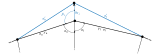
\includegraphics{img/model_development/node_shift_normal}
        \caption{Normal Direction}
        \label{fig:model_development/surface_normal}
    \end{subfigure}%
    \begin{subfigure}{0.5\linewidth}
        \centering
        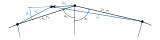
\includegraphics{img/model_development/node_shift_tangential}
        \caption{Tangential Direction}
        \label{fig:model_development/surface_tangential}
    \end{subfigure}
    \caption{Shifting of Surface Nodes}
    \label{fig:surface-node-shifting}
\end{figure}

\begin{figure}
    \begin{subfigure}{\linewidth}
        \centering
        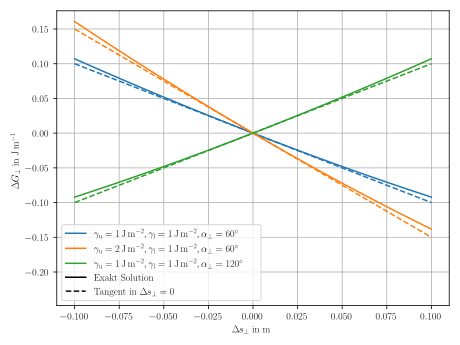
\includegraphics{img/model_development/plot_normal_potential}
        \caption{Normal Direction}
        \label{fig:model_development/plot_normal_potential}
    \end{subfigure}
    \begin{subfigure}{\linewidth}
        \centering
        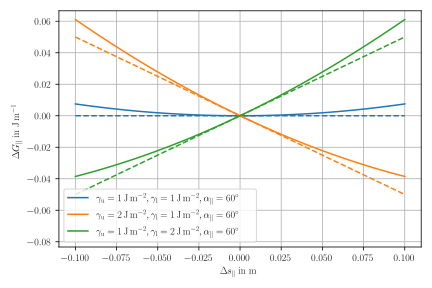
\includegraphics{img/model_development/plot_tangential_potential}
        \caption{Tangential Direction}
        \label{fig:model_development/plot_tangential_potential}
    \end{subfigure}
    \caption{Change in Gibbs Energy Due to Node Shifting (tangents dashed)}
    \label{fig:surface-node-potentials}
\end{figure}

If a node is displaced (shifted) in space, a change in Gibbs energy occurs due to the change in surface resp.\ interface area.
The amount of energy bound in a surface or interface is described by the interface energy $\InterfaceEnergy$.
Since a 2D problem is regarded, the length of the surface line $\SurfaceDistance$ is a measure of present surface area.
The change of Gibbs energy due to node shifting is described by \autoref{eq:gibbs-diff-surface-normal} with the prime values as measures after shifting.

\begin{equation}
    \Step\Normal\GibbsEnergy = \left( \Upper\SurfaceDistance' - \Upper\SurfaceDistance + \Lower\SurfaceDistance' - \Lower\SurfaceDistance \right) \Surface{\InterfaceEnergy}
    \label{eq:gibbs-diff-surface-normal}
\end{equation}

The shifting of nodes is separated into two components as shown in \autoref{fig:surface-node-shifting}.
The normal vector points under an angle of $\Normal\SurfaceVectorAngle$ acc.~to~\autoref{eq:delta-surface-normal} to both surface lines.

\begin{equation}
    \Normal\SurfaceVectorAngle = \pi - \frac{1}{2} \left(\Upper\SurfaceRadiusAngle + \Lower\SurfaceRadiusAngle\right)
    \label{eq:delta-surface-normal}
\end{equation}

With a certain normal shift $\Normal{\Step\Shift}$, the surface lengths after shifting are calculated by \autoref{eq:surface-distance-shifted-normal-upper} and \autoref{eq:surface-distance-shifted-normal-lower}.

\begin{align}
    \Upper\SurfaceDistance' &= \sqrt{\Upper{\SurfaceDistance}^2 + \Normal{\Step\Shift}^2 - 2 \Upper{\SurfaceDistance} \Normal{\Step\Shift} \cos \Normal\SurfaceVectorAngle} \label{eq:surface-distance-shifted-normal-upper}\\
    \Lower\SurfaceDistance' &= \sqrt{\Lower{\SurfaceDistance}^2 + \Normal{\Step\Shift}^2 - 2 \Lower{\SurfaceDistance} \Normal{\Step\Shift} \cos \Normal\SurfaceVectorAngle} \label{eq:surface-distance-shifted-normal-lower}
\end{align}

The slope of the tangent in $\Normal{\Step\Shift} = 0$ is calculated as in \autoref{eq:gibbs-partial-surface-normal}.
\autoref{fig:model_development/plot_normal_potential} shows the change in Gibbs energy due to normal shifting with different values of $\Normal\SurfaceVectorAngle$ and $\InterfaceEnergy$.
A $\Normal\SurfaceVectorAngle > \qty{90}{\degree}$ means a convex surface, thus energy gain when inward shifting (negative $\Normal{\Step\Shift}$).
A $\Normal\SurfaceVectorAngle < \qty{90}{\degree}$ means a concave surface, thus energy gain when outward shifting (positive $\Normal{\Step\Shift}$).
A $\Normal\SurfaceVectorAngle = \qty{90}{\degree}$ means a even surface, thus energy loss in both shifting directions.
Note, that the slope is dependent on the sum of $\Upper{\InterfaceEnergy}$ and $\Lower{\InterfaceEnergy}$, whereas the monotonicity depends on $\Normal\SurfaceVectorAngle$.

\begin{equation}
    \frac{\partial \GibbsEnergy}{\partial \Normal{\Shift}} = \lim_{\Step\Normal\Shift \rightarrow 0} \frac{\Step\Normal\GibbsEnergy}{\Step\Normal\Shift} = -\left(\Upper{\InterfaceEnergy} + \Lower{\InterfaceEnergy}\right) \cos \Normal\SurfaceVectorAngle
    \label{eq:gibbs-partial-surface-normal}
\end{equation}

\begin{equation}
    \frac{\partial \Volume}{\partial \Normal{\Shift}} = \frac{1}{2} \left( \Upper\SurfaceDistance + \Lower\SurfaceDistance \right) \sin \Normal\SurfaceVectorAngle
    \label{eq:volume-partial-surface-normal}
\end{equation}

Regarding the normal shifting, the direction vector is under an angle of $\Tangential\SurfaceVectorAngle$ acc.~to.~\autoref{eq:delta-surface-tangential} to the upper surface line.

\begin{equation}
    \Tangential\SurfaceVectorAngle = \Normal\SurfaceVectorAngle - \frac{\pi}{2}
    \label{eq:delta-surface-tangential}
\end{equation}

The change in Gibbs energy is calculated in a similar way acc.~to~\autoref{eq:gibbs-diff-surface-tangential}, but the shifted surface lengths calculate as in \autoref{eq:surface-distance-shifted-tangential-upper} and \autoref{eq:surface-distance-shifted-tangential-lower} in dependence on the tangential shift $\Tangential{\Step\Shift}$.
Note the signs before the cosine terms.

\begin{equation}
    \Step\Normal\GibbsEnergy = \left( \Upper\SurfaceDistance' - \Upper\SurfaceDistance + \Lower\SurfaceDistance' - \Lower\SurfaceDistance \right) \Surface{\InterfaceEnergy}
    \label{eq:gibbs-diff-surface-tangential}
\end{equation}

\begin{align}
    \Upper\SurfaceDistance' &= \sqrt{\Upper{\SurfaceDistance}^2 + \Tangential{\Step\Shift}^2 - 2 \Upper{\SurfaceDistance} \Tangential{\Step\Shift} \cos \Tangential\SurfaceVectorAngle} \label{eq:surface-distance-shifted-tangential-upper} \\
    \Lower\SurfaceDistance' &= \sqrt{\Lower{\SurfaceDistance}^2 + \Tangential{\Step\Shift}^2 + 2 \Lower{\SurfaceDistance} \Tangential{\Step\Shift} \cos \Tangential\SurfaceVectorAngle} \label{eq:surface-distance-shifted-tangential-lower}
\end{align}

The slope of the tangent in $\Tangential{\Step\Shift} = 0$ is calculated as in \autoref{eq:gibbs-partial-surface-tangential}.
\autoref{fig:model_development/plot_tangential_potential} shows the change in Gibbs energy due to normal shifting with different values of $\InterfaceEnergy$.
The slope and monotonicity of these curves is here dependent on the \emph{difference} of $\Upper{\InterfaceEnergy}$ and $\Lower{\InterfaceEnergy}$.
The convexity or concavity of the surface is here only of minor importance.
Whether the interface with higher $\InterfaceEnergy$ is located on the upper or lower side determines the monotonicity of the curves.
In the special case when $\Upper{\InterfaceEnergy} = \Lower{\InterfaceEnergy}$, the curve has a minimum in $\Tangential{\Step\Shift} = 0$, meaning that any shift will produce an energy loss.
This is the case on all nodes except neck nodes.

\begin{equation}
    \frac{\partial \GibbsEnergy}{\partial \Tangential{\Shift}} = \lim_{\Step\Tangential\Shift \rightarrow 0} \frac{\Step\Tangential\GibbsEnergy}{\Step\Tangential\Shift} = -\left(\Upper{\InterfaceEnergy} - \Lower{\InterfaceEnergy}\right) \cos \Tangential\SurfaceVectorAngle
    \label{eq:gibbs-partial-surface-tangential}
\end{equation}

\begin{equation}
    \frac{\partial \Volume}{\partial \Tangential{\Shift}} = \frac{1}{2} \left( \Lower\SurfaceDistance - \Upper\SurfaceDistance \right) \sin \Tangential\SurfaceVectorAngle
    \label{eq:volume-partial-surface-tangential}
\end{equation}